\chapter{Client Server Communication}
There are some issues to design a communication system for client-server architecture, such as \textbf{addressing, primitives, protocols and reliability.}

\section{Addressing}
Addressing refers to the ability of a client to \textbf{understand where the server is (server localization)}. There can be different solutions to solve these problems and answers to questions like \textit{"Where is the server?".}

\subsection{LAN}
The assumption that \textbf{client knows the address of the server and server gets also the address of the client} when it receives a request. The problem of this solution is that \textbf{there is no location transparency} and in case of relocating to the server it is necessary to apply modification on the client.
\begin{figure}[!h]
            \centering
            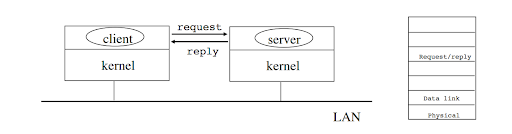
\includegraphics[width=.7\linewidth]{images/clientServerCommunication/clientServerLan.png}
            \caption{Client Server LAN}
    \end{figure}

\subsection{Broadcast}
\begin{enumerate}
    \item Client sends via broadcast a \textbf{special packet} \textit{"locate"} to identify the server and discover where it is located
    \item Only the server answers \textit{“I Am Here”} with his physical address
    \item The client send the \textit{"request"} to that address
    \item The server sends a \textit{"reply"} to the client
    \item This solution \textbf{offers location transparency.} The \textbf{problem} regards the \textit{usage of channels}, since now there is an \textbf{increasing amount of traffic} due to broadcast flooding.
\end{enumerate}
\begin{figure}[!h]
            \centering
            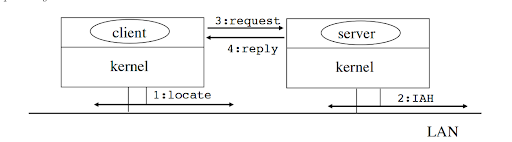
\includegraphics[width=.7\linewidth]{images/clientServerCommunication/clientServerBroadcast.png}
            \caption{Client Server Broadcast}
    \end{figure}

\subsection{Usage of Name Server}
It provides mapping of local names of the servers and physical addresses:
\begin{enumerate}
    \item The client sends to NS a message \textit{"lookup"} to get the server address
    \item The NS answer with a \textit{"replay"} message with the physical address of the server
    \item The client sends a \textit{"request"} to the server
    \item The server sends a \textit{"reply"} to the client
\end{enumerate}
\begin{figure}[!h]
            \centering
            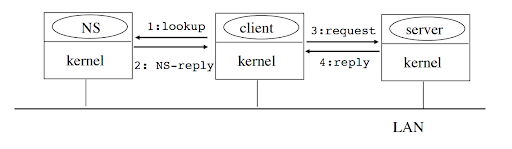
\includegraphics[width=.7\linewidth]{images/clientServerCommunication/clientServerNS.png}
            \caption{Client Server Name Server}
    \end{figure}
\begin{itemize}
    \item This solution \textbf{provides location transparency} for the \textit{server}
    \item But it does \textbf{not provide location transparency} for the \textit{NS} since for each communication the client has to contact the NS, so that could be considered as a bottleneck.
    \item Possible replication for robustness, since it is hard to keep consistency of the copies
\end{itemize}

\subsection{Primitives / Operations}
\begin{enumerate}
    \item \textbf{Synchronous:} processes are blocked when they use primitives.
        \begin{itemize}
            \item \textit{Send:}
                \begin{itemize}
                    \item It specifies the \textbf{send buffer} and the \textbf{destination address}
                    \item Process remains \textbf{blocked} until the buffer has been sent.
                \end{itemize}
            \item \textit{Receive:}
                \begin{itemize}
                    \item The invocation does not return control to the calling process until the message has been received and deposited into a destination buffer specified from the calling
                \end{itemize}
        \end{itemize}
    \item \textbf{Asynchronous:}
        \begin{itemize}
            \item \textit{Send:}
                \begin{itemize}
                    \item The control returns to the process as soon as the buffer to be sent is \textbf{copy into the buffer of the kernel (local)}
                    \item Process is blocked just the time it takes to copy the message inside the buffer.
                \end{itemize}
            \item \textit{Receive:}
                \begin{itemize}
                    \item Indicates to the kernel the local base address and the size of the buffer where data is received
                    \item It returns control to the calling process.
                \end{itemize}
            \item \textit{Advantages:} the caller \textbf{continues the computation} concurrently to the communication
            \item \textit{Disadvantage:} it is difficult to \textbf{recognize when the communication is terminated.} How can we migrate this problem?
                \begin{itemize}
                    \item Implement an \textbf{alternative} to asynchronous send
                        \begin{itemize}
                            \item The \textbf{buffer} to be sent is in the \textbf{process space} \(\rightarrow\) the caller cannot change it until it is transmitted
                            \item The \textbf{buffer} to be sent is in the \textbf{kernel space} \(\rightarrow\) cost of copying
                        \end{itemize}
                    \item \textbf{Interrupt} from the core when the buffer has been transmitted
                        \begin{itemize}
                            \item Does not require copying
                            \item The sender can reuse the buffer after the interrupt
                        \end{itemize}
                \end{itemize}
        \end{itemize}
    \item \textbf{Primitives with buffer:} receiver has a buffer in which it can \textbf{store messages} sent by sender and it can be introduced in synchronous and asynchronous systems:
        \begin{itemize}
            \item The process that invokes the receive, \textbf{asks the kernel to create the mailbox} and specifies its local address (ex: port number)
            \item The kernel keeps the mailbox in the kernel space
            \item Messages arrive with the process address and are put in the mailbox
                \begin{itemize}
                    \item If there is a \textbf{pending receive} the message is passed to the process, eventually unblocking it, otherwise the message is kept until an invocation does not arrive.
                \end{itemize}
            \item If the mailbox is full the kernel could discard the message \(\rightarrow\) \textbf{message loss event}
        \end{itemize}
    \item \textbf{Primitives without buffer:} so the communications \textbf{must be synchronous}, sender is blocked until it receives an unblock
        \begin{itemize}
            \item The \textbf{caller is blocked} when it invokes the \textit{"receive(addr, \&m)"}, where addr is the address of the sending process and \&m is the memory space of the invoking process
            \item Kernel unblocks the caller when message is received and copied in the buffer
            \item If the \textbf{message is received} and there are \textbf{no more pending} \textit{"receive"}, the kernel cancels the message and the client tries again
            \item If the \textit{"receive"} is from a server that is executing operations for a client and another client sends a message, there is a \textbf{race condition} since the new client has to wait for a new receive from the server
        \end{itemize}
\end{enumerate} 

\section{Protocols}
\textbf{Fragmentation} and \textbf{re-composition} of messages might be needed at application level if the message is too long. Messages will be split in \textbf{packets}.

\begin{figure}[h]
            \centering
            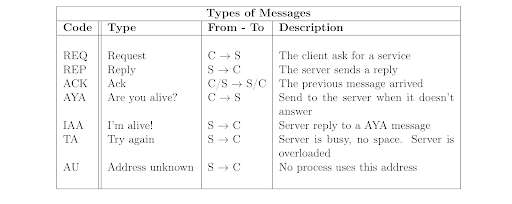
\includegraphics[width=.9\linewidth]{images/clientServerCommunication/addressingTable.png}
    \end{figure}
\textbf{Ack} from \textbf{server} to client can be \textbf{useful to get some information} about the communication or execution performance and it allows the client to send another request. Instead \textbf{ack} from \textbf{client} to server can be useful to distinguish requests and discard copies of replies.
\begin{itemize}
    \item \textbf{AYA, IAA:} if a client sends a request and the answer \textbf{does not come back} in a given time: is the server working properly?
        \begin{itemize}
            \item The client sends a message AYA to test the server if the answer is a message IAA or REP, ok, otherwise it sends again an AYA after some attempts it can assume that the server is not alive
        \end{itemize}
    \item \textbf{TA:} sometime the server \textbf{cannot accept a REQ}, thus:
        \begin{itemize}
            \item The server does not have buffer space for new message
            \item The server is overloaded
        \end{itemize}
    \item \textbf{AU:} mistake in the address \(\rightarrow\) the client has not to try again
    \begin{figure}[!h]
            \centering
            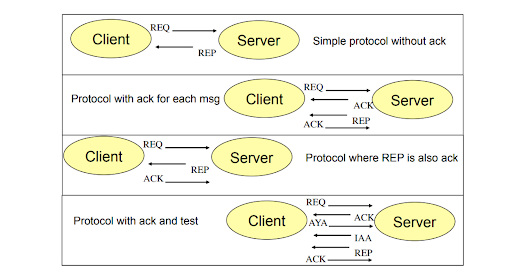
\includegraphics[width=.7\linewidth]{images/clientServerCommunication/exampleInteraction.png}
            \caption{Examples of interaction Client-Server}
    \end{figure}
\end{itemize}

\section{Networks / Reliability}
Communication in distributed system depends on the usage of a network that connects computer systems. Networks can be distinguished considering their size (LAN, MAN, WAN) or transmission technology (wired, wireless), and the different level of QoS offered. In this case the QoS provided by a network takes care of its performances (transmission speed, latency, band), reliability and security. The implementation of a distributed system has to consider also this aspect, for instance latency is useful for the development of synchronous systems. Distributed Systems are mainly implemented on application level.
\begin{figure}[!h]
            \centering
            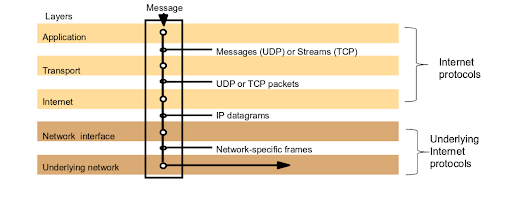
\includegraphics[width=.7\linewidth]{images/clientServerCommunication/networkReliability.png}
            \caption{Networks / Reliability}
    \end{figure}